\section{Résultats et discussion}\label{sec:res}
\subsection{Données recueillies}
La campagne comprend 2\,250 essais (5 technologies $\times$ 5 fonctionnalités $\times$ 3 niveaux de charge $\times$
30 essais), soit 1,8 million de requêtes mesurées et 225\,000 requêtes de chauffe. Aucune requête n'a échoué. Le
fichier brut contient une ligne par essai (18 colonnes : débit, latences, CPU, mémoire, démarrage). D'un essai à
l'autre, le débit varie en médiane de 9,7\,\% (écart-type rapporté à la moyenne) et jusqu'à 17,6\,\% : les écarts
inférieurs à environ 15\,\% ne se lisent donc pas sur un essai isolé, et les comparaisons ci-dessous reposent sur
les 30 essais (test de Mann-Whitney deux à deux, correction de Holm). Sauf mention contraire, les valeurs sont
données pour 50 utilisateurs simultanés.

\begin{table}[t]
\caption{Débit moyen (requêtes/s) à 50 utilisateurs, 30 essais par case}\label{tab:debit}
\centering\small
\begin{tabular}{@{}lrrrrr@{}}
\toprule
\textbf{Techno.} & \textbf{F1} & \textbf{F2} & \textbf{F3} & \textbf{F4} & \textbf{F5}\\
\midrule
Rust & 13\,373 & 7\,735 & 806 & 9\,261 & 243 \\
Go & 7\,517 & 5\,820 & 761 & 6\,791 & 237 \\
PHP & 6\,488 & 5\,500 & 721 & 6\,335 & 230 \\
Node.js & 4\,792 & 4\,003 & 752 & 4\,186 & 271 \\
Python & 1\,433 & 1\,443 & 535 & 1\,468 & 242 \\
\bottomrule
\end{tabular}
\end{table}

\begin{table}[t]
\caption{Latence, CPU, mémoire et démarrage (50 utilisateurs)}\label{tab:synth}
\centering\small
\setlength{\tabcolsep}{3.5pt}
\begin{tabular}{@{}lrrrrr@{}}
\toprule
 & \textbf{p95 F2} & \textbf{CPU F1} & \textbf{CPU F5} & \textbf{Mém.} & \textbf{Démar.}\\
\textbf{Techno.} & {\scriptsize(ms)} & {\scriptsize(ms/req)} & {\scriptsize(ms/req)} & {\scriptsize(Mo)} & {\scriptsize(ms)}\\
\midrule
Rust & 11,1 & 0,06 & 4,08 & 9 & 6 \\
Go & 15,9 & 0,11 & 4,18 & 18 & 7 \\
PHP & 23,2 & 0,13 & 4,29 & 42 & 30 \\
Node.js & 22,3 & 0,18 & 3,67 & 53 & 41 \\
Python & 40,8 & 0,68 & 4,11 & 33 & 160 \\
\bottomrule
\end{tabular}
\end{table}

\subsection{Analyse}
\paragraph{Débit.} La figure~\ref{fig:debit} et le tableau~\ref{tab:debit} montrent un classement net sur les
fonctionnalités légères. En création (F1), Rust traite 13\,373 requêtes/s (intervalle de confiance à 95\,\% :
$\pm$567), contre 7\,517 pour Go, 6\,488 pour PHP, 4\,792 pour Node.js et 1\,433 pour Python : Rust est 9,3 fois plus
rapide que Python. Les rapports Rust/Python sont de 5,4 en liste (F2) et de 6,3 en jointure (F4). Les dix paires de
technologies diffèrent significativement pour F1, F2 et F4. Pour la recherche (F3), l'écart se réduit à 1,5 entre
Rust (806) et Python (535), et Go et PHP ne se distinguent pas statistiquement de Node.js (Go--Node.js :
$p=0{,}51$ ; PHP--Node.js : $p=0{,}07$). Pour les statistiques (F5), les cinq versions se situent entre 230 et
271 requêtes/s ; Rust et Python sont indiscernables ($p=0{,}68$) et Node.js est de 12 à 18\,\% au-dessus des autres.

\begin{figure}[t]
\centering
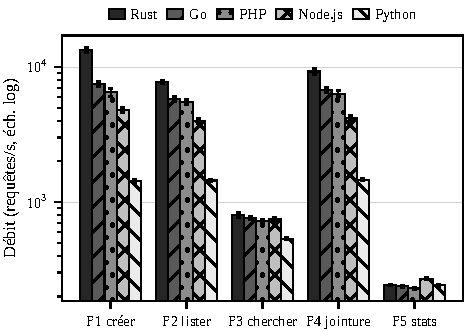
\includegraphics[width=\columnwidth]{figures/fig_debit.pdf}
\caption{Débit par fonctionnalité à 50 utilisateurs (barres : intervalle de confiance à 95\,\%, 30 essais).}
\label{fig:debit}
\end{figure}

\paragraph{Évolution avec la charge.} Le débit reste presque constant de 10 à 100 utilisateurs (par exemple Python
en F1 : 1\,445, 1\,433 et 1\,450 requêtes/s) : le cœur du serveur est déjà saturé dès 10 utilisateurs. Comme les
utilisateurs envoient une requête dès la réponse reçue, la latence moyenne vaut à peu près le nombre d'utilisateurs
divisé par le débit (loi de Little) et croît donc proportionnellement. La latence p95 de F1 (figure~\ref{fig:charge1})
passe de 12,9 à 80,0\,ms pour Python (+67\,ms) et de 1,9 à 17,8\,ms pour Rust (+16\,ms) entre 10 et 100 utilisateurs.

\begin{figure}[t]
\centering
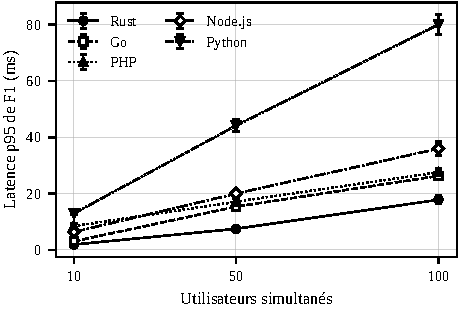
\includegraphics[width=\columnwidth]{figures/fig_charge_create.pdf}
\caption{Latence p95 de la création (F1) selon le nombre d'utilisateurs simultanés.}
\label{fig:charge1}
\end{figure}

\paragraph{Latences extrêmes.} En F5, les latences médianes des cinq versions sont proches (175 à 210\,ms), mais la
latence p95 de Rust atteint 396\,ms, contre 215 à 275\,ms pour les autres (figure~\ref{fig:charge5}). À 100
utilisateurs, elle est de 846\,ms pour Rust et de 405 à 577\,ms pour les autres. Une moyenne seule aurait caché cette
différence.

\begin{figure}[t]
\centering
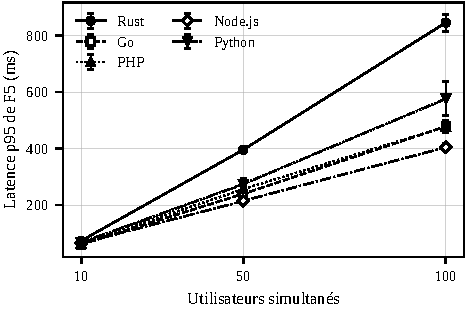
\includegraphics[width=\columnwidth]{figures/fig_charge_stats.pdf}
\caption{Latence p95 des statistiques (F5) selon le nombre d'utilisateurs simultanés.}
\label{fig:charge5}
\end{figure}

\paragraph{Coût en processeur.} La figure~\ref{fig:cpu} montre le temps CPU consommé par requête. En F1, Python
dépense 0,68\,ms, soit 11 fois plus que Rust (0,06\,ms), Go (0,11), PHP (0,13) et Node.js (0,18) se situant entre les
deux. En F3 et F5, ce coût est de 1,2 à 1,8\,ms et de 3,7 à 4,3\,ms pour toutes les versions : l'essentiel est
dépensé par SQLite.

\begin{figure}[t]
\centering
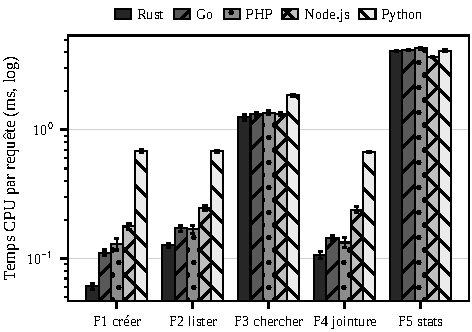
\includegraphics[width=\columnwidth]{figures/fig_cpu.pdf}
\caption{Temps CPU du serveur par requête, à 50 utilisateurs (échelle logarithmique).}
\label{fig:cpu}
\end{figure}

\paragraph{Mémoire et démarrage.} Rust occupe 8,5\,Mo et démarre en 6\,ms, Go 17,6\,Mo et 7\,ms. Python (33,5\,Mo,
160\,ms), PHP (41,7\,Mo pour ses cinq processus, 30\,ms) et Node.js (52,9\,Mo, 41\,ms) viennent ensuite
(figure~\ref{fig:mem}, tableau~\ref{tab:synth}).

\begin{figure}[t]
\centering
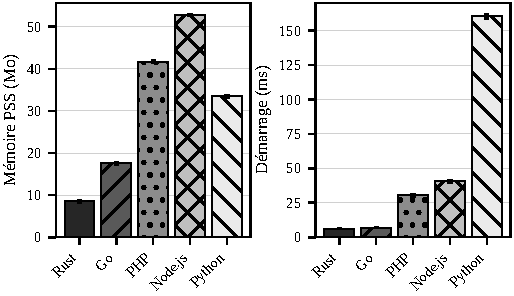
\includegraphics[width=0.92\columnwidth]{figures/fig_memoire_demarrage.pdf}
\caption{Mémoire (PSS en fin d'essai) et temps de démarrage, moyennes sur tous les essais.}
\label{fig:mem}
\end{figure}

\subsection{Interprétation et discussion}
\textbf{H1 est confirmée en grande partie.} Sur F1, F2 et F4, l'ordre Rust, Go, PHP, Node.js, Python est respecté et
chaque paire est significativement différente. Notre hypothèse plaçait pourtant PHP et Node.js au même niveau : PHP
est en réalité meilleur (par exemple 6\,488 contre 4\,792 requêtes/s en F1), avec un coût CPU par requête plus faible
(0,13 contre 0,18\,ms). Nous n'avons pas isolé la cause ; l'hypothèse la plus simple est que le chemin d'une requête
(analyse HTTP, décodage de l'URL, JSON) est plus court dans le serveur intégré de PHP, écrit en C, que dans les
couches JavaScript de Node.js.

\textbf{H2 est confirmée.} En F5, le CPU mesuré par requête (3,7 à 4,3\,ms) est proche du temps des deux requêtes SQL
exécutées seules, sans HTTP : 3,4\,ms dans Node.js (SQLite 3.53.4), 3,7 dans Python (3.53.1) et 4,2 dans PHP
(3.45.1). Le surcoût propre à la technologie ne représente que quelques dixièmes de milliseconde. Le léger avantage
de Node.js en F5 est cohérent avec un moteur SQLite plus récent, mais Python a la même version 3.53 sans cet avantage
et nous ne pouvons pas séparer les deux effets.

\textbf{H3 est partiellement confirmée.} La latence extrême croît bien avec la charge pour toutes les versions, et
l'augmentation absolue est la plus forte pour Python. En valeur relative, c'est pourtant Rust qui varie le plus (la
p95 de F1 est multipliée par 9,4, contre 6,2 pour Python), car sa latence à faible charge est très petite. Pour la
p95 de F5, Rust est le moins bon : nous supposons que les 50 fils d'exécution se disputent les quatre connexions
SQLite sans ordre d'attente équitable (verrou et variable de condition), mais ce point n'a pas été vérifié.

\textbf{H4 est partiellement confirmée.} Rust et Go sont les moins gourmands et les plus rapides au démarrage, mais
les technologies interprétées ne sont pas toutes plus lourdes : Python consomme moins de mémoire que PHP et Node.js.

\textbf{Portée.} Un facteur 9 n'a d'effet que si le serveur est saturé : à 1\,433 requêtes/s, la version Python sert
déjà, à titre d'ordre de grandeur, plus de 100 millions de requêtes par jour sur un seul cœur. Dès que SQLite travaille
(F3, F5), changer de langage apporte peu : l'effort doit alors porter sur la requête et l'index.

\textbf{Limites.} (i)~Nous comparons cinq implémentations, pas cinq langages : les versions Go et Rust utilisent
un serveur rudimentaire, et Flask et \texttt{php -S} sont des serveurs de développement. (ii)~Chaque serveur est limité
à un cœur ; le gain du parallélisme n'est pas mesuré. (iii)~Les versions de SQLite diffèrent (3.53 pour Python et
Node.js, 3.45.1 pour les autres). (iv)~Le client et le serveur communiquent sur la même machine, sans réseau, dans un
conteneur partagé à deux cœurs : les valeurs absolues ne se transposent pas à une autre machine, seules leurs
proportions sont instructives. (v)~La base (10\,000 lignes) tient en mémoire et chaque essai compte 500 ou 1\,000
requêtes. (vi)~Nous n'avons pas testé d'autres frameworks ni d'autres bases de données.
